\documentclass{src/thesis}  % uncomment for writing
% \documentclass[print]{src/thesis} % uncomment for printing version

% ------------------- PACKAGES ------------------- %
\usepackage{amsmath}        %Used for math
\usepackage{amsthm}         %Used for intermezzos
\usepackage{lipsum}         %Used for dummy text
\usepackage{longtable}      %Used to put nomenclature on multiple pages
\usepackage{multicol}       %For multiple columns in table
\usepackage{multirow}       %For multiple rows in table
\usepackage{tcolorbox}      %For statements and contributions
\usepackage{thmtools}       %For declaring theorems
\usepackage{todonotes}      %For to do notes
%\usepackage{tikz}          %The tikz package is added in mrthesis.cls for producing thumbindex
\usepackage{url}            %To provide urls in the document
\usepackage[hidelinks]{hyperref} %For hyperlinks in the document
\usepackage{bookmark}       %Works with hyperref to setup styles and colors
\usepackage{enumitem}       %To shift items in itemize left
\usepackage{wrapfig}        %To wrap text around a figure






% ------------------- PREAMBLE ------------------- %
% Counters
\newcounter{ContNum}        % Counter for the contributions
\renewcommand{\theContNum}{\Roman{ContNum}}

%Other commands
\newcommand{\itemheader}[1]{~\\ \noindent\textbf{#1.}\ \ }%
\newcommand{\itemheaderNewpage}[1]{\newpage \noindent\textbf{#1.}\ \ }%
\newcommand{\contribution}[2]{\refstepcounter{ContNum}#2 \vspace*{2.1mm}\begin{tcolorbox}[colback=black!2!white,colframe=black!20!white] \textbf{Contribution \Roman{ContNum}.} {\em #1} \end{tcolorbox}\vspace*{2.1mm}}
\newcommand{\objective}[1]{\begin{tcolorbox}[colback=black!2!white,colframe=black!20!white] {\em #1} \end{tcolorbox}}
\newcommand{\terminology}[2]{\begin{tcolorbox}[colback=black!2!white,colframe=black!20!white] {\textbf{Terminology: } \textbf{#1} \em #2} \end{tcolorbox}}

% Define the cover count counter
\newcounter{covercount}

% Redefine the \cover command
\newcommand{\cover}[1]{%
  \ifprint{}%
  \else%
    \stepcounter{covercount}%
    \includepdf[pages=-]{#1}%
    \ifnum\value{covercount}=1
      \cleardoublepage%
    \fi%
  \fi%
}

% To create a blank footnote:
\newcommand\blfootnote[1]{%
  \begingroup
  \renewcommand\thefootnote{}\footnote{#1}%
  \addtocounter{footnote}{-1}%
  \endgroup
  \vspace{-0.4cm} %correct for the whitespace it occupies
}


% Referring to the Modifications chapter:
\newcommand{\disclaimer}{\\[\baselineskip]  A detailed list of the differences between this chapter and the article on which it is based is provided in the \hyperref[chap: Modifications]{\textit{Modifications}} chapter of this thesis.}
%!TEX root = ../thesis.tex
\usepackage{tikz}
\usepackage{pgfplots}
% and optionally (as of Pgfplots 1.3):
\pgfplotsset{compat=newest}
\pgfplotsset{plot coordinates/math parser=false}
\newlength\figureheight
\newlength\figurewidth

\usepackage[utf8]{inputenc}
\usepackage{pgfgantt}
\usepackage{pdflscape}
\pgfplotsset{compat=newest}
\pgfplotsset{plot coordinates/math parser=false}

% %% the following commands are needed for some matlab2tikz features
\usetikzlibrary{plotmarks}
\usetikzlibrary{arrows.meta}
\usepgfplotslibrary{patchplots}

\newcommand{\SF}{1}                 % Scaling factor
\newcommand{\TS}{\normalsize}       % Text size
\newcommand{\lw}{0.7pt}             % Line width
\newcommand{\TSTick}{\small}        % Text size axis labels
\newcommand{\axislabels}[2]{\foreach \x/\y/\s in {#1} {\node[#2,inner sep=1mm] at (\x,\y) {\TSTick $\s$};}}
\newcommand{\wheel}[3]{ \draw[line width=\lw] (#1,#2) circle (#3);
                        \fill[bottom color=MRblue!60!black!80,top color=MRblue!10] (#1,#2) circle (#3-0.5*\lw);
                        \fill[color=MRblue!30] (#1,#2) circle (#3-\lw);
                        \fill[top color=MRblue!60!black!80,bottom color=MRblue!10] (#1,#2) circle (0.7*#3);
                        \fill[color=MRblue!30] (#1,#2) circle (0.7*#3-\lw);
                        \fill[color=black] (#1,#2) circle (0.1*#3);}

\newcommand{\CoM}[3]{\filldraw[inner color=white,outer color=black!7!white,draw=black,line width=\lw] (#1,#2) circle (#3+0.5*\lw);
                     \begin{scope}[xshift=#1,yshift=#2]
                        \clip(-#3,0) -- (0,0) -- (0,#3) -- (#3,#3) -- (#3,0) -- (0,0) -- (0,-#3) -- (-#3,-#3) -- cycle;
                        \fill[inner color=black!50!white,outer color=black] (0,0) circle (#3);
                     \end{scope}}
\usetikzlibrary{arrows}
\usetikzlibrary{patterns}
\usetikzlibrary{decorations.markings}
\usetikzlibrary{shadings}
\usetikzlibrary{shapes}


\declaretheorem[name={Remark},style=plain,numberwithin=chapter]{rmk}
\declaretheorem[name={Definition},style=definition,numberwithin=chapter]{dfn}
\declaretheorem[name={Theorem},qed=$\blacktriangle$,style=plain,numberwithin=chapter]{thm}
\declaretheorem[name={Lemma},qed=$\blacktriangle$,style=plain,numberwithin=chapter]{lem}
\declaretheorem[name={Assumption},style=definition,numberwithin=chapter]{asm}
\declaretheorem[name={Property},style=plain,numberwithin=chapter]{prop}
\declaretheorem[name={Example},style=plain,numberwithin=chapter]{example}
\declaretheorem[name={Corollary},qed=$\blacktriangle$,style=plain,numberwithin=chapter]{cor}
\declaretheorem[name={Intermezzo},style=definition,numberwithin=chapter]{intermez}

\graphicspath{{img/}{../../img/}{../../../img/}}


% ------------------- Document colors -------------------%
% DEEP BLUE
\definecolor{thumbcolor}{RGB}{4,51,83} %{250,180,140}
\definecolor{deepcolor}{RGB}{0,0,0}
\definecolor{titlecolor}{RGB}{4,51,83}%{238,112,35}


% ------------------- Document Details -------------------%
%Author details
\author{Author Name}
\newcommand{\placeofbirth}{Birthplace}

%Defense details
\newcommand{\defensedate}{maandag 30 december 2022}
\newcommand{\defensetime}{16:00}
\newcommand{\rector}{prof. dr. Rector}

%Thesis details
\newcommand{\maintitle}{Awesome thesis title}
\newcommand{\subtitle}{with an awesome subtitle}
\newcommand{\isbn}{123-45-678-9012-3}     % 123boldmath-45-678-9012-3
\newcommand{\printer}{Name of printer || www.printerswebsite.nl}
\newcommand{\designer}{Name of cover designer}
\newcommand{\project}{Here you can put the acknowledgment in case this thesis is partially 
supported by the Research Project XXX through the European Union H2020 
program under GA XXXXXX.}

%Details about the committee (note that there should be NO space between titles (prof.dr.)
\newcommand{\chair}{prof.dr. Name Surname}
\newcommand{\promotor}{prof.dr. Name Surname}
\newcommand{\copromotor}{prof.dr. Name Surname}
\newcommand{\firstmember}{prof.dr. Name Surname}
\newcommand{\secondmember}{prof.dr. Name Surname}
\newcommand{\thirdmember}{prof.dr. Name Surname}
\newcommand{\fourthmember}{prof.dr. Name Surname}
% other relevant meta data about the thesis can be found in preface.tex

\makeatletter % generates all the \author stuff

\begin{document} 
\pagenumbering{roman}
\thispagestyle{empty}

% ------------------- Front Cover -------------------%
% \cover{thesis_front.pdf}    % Adds your thesis' front cover if the option 'print' is NOT used. Printing companies require the thesis cover to be supplied separately and in a different format. Definition of \cover{} is given in commands.tex.

% ------------------- First Sections -------------------%
% ---------------- First page: title and name ---------------- %
\thispagestyle{empty}
\vspace*{30mm}\noindent
\begin{center}
{\LARGE\sf\maintitle}\\[4.5cm] %\\[7mm]
{\Large\sf \@author}
\end{center}

\newpage
\thispagestyle{empty}






% --------------- Second page: acknowledgments --------------- %
%TUE logo 
\vspace*{\fill}
\noindent
\includegraphics[width=5cm]{img/TUE-logo.pdf}\\
{\small The work described in this thesis was carried out at the Eindhoven University of
Technology.}\\[8mm]

% Project Logo %
\noindent
\includegraphics[width=5cm]{img/ProjectLogo.pdf}\\[2mm]
\noindent\bgroup\small\project
\\[8mm]

%ISBN%
\noindent\bgroup\small
A catalogue record is available from the Eindhoven University of Technology Library.\\
ISBN: \isbn\\[4mm]

%Other%
Typeset by the author using the pdf \LaTeX \ documentation system.\\
Cover design: \designer \\
Reproduction: \printer\\[8mm]
\copyright\year \ by \@author. All rights reserved.}
\egroup

\newpage
\thispagestyle{empty}





% ------------------- Third page: Title page ------------------- %
\vspace*{30mm}
\begin{center}
{\LARGE\sf\maintitle}\\[30mm] %\\[7mm]
{\large\textsc{Proefschrift}}\\[8mm]
ter verkrijging van de graad van doctor aan de\\
Technische Universiteit Eindhoven, op gezag van de\\
rector magnificus \rector, voor een\\
commissie aangewezen door het College voor\\
Promoties, in het openbaar te verdedigen\\
op \defensedate\ om \defensetime\ uur\\[8mm]
door\\[8mm]
\@author\\[8mm]
geboren te \placeofbirth
\end{center}
\vfill

\newpage
\thispagestyle{empty}

\noindent
Dit proefschrift is goedgekeurd door de promotoren en de samenstelling van de promotiecommissie is als volgt:\\[7mm]

\noindent
\begin{tabular}{@{}l p{9.8cm}}
voorzitter:                 &   \chair        \\                \\
promotor:                   &   \promotor     \\
co-promotor:                &   \copromotor   \\
leden:                      &   \firstmember  \\
                            &   \secondmember \\
                            &   \thirdmember  \\
                            &   \fourthmember \\
\end{tabular}

\vfill
\noindent
Het onderzoek dat in dit proefschrift wordt beschreven is uitgevoerd in overeenstemming met de TU/e Gedragscode Wetenschapsbeoefening.

\chapter*{Summary} % Try to keep within approx 350 words / one page
\addcontentsline{toc}{chapter}{Summary}
\markboth{Summary}{Summary}


\begin{center}
\rule{\textwidth}{.75pt}\vspace*{1mm}
\textbf{{\Large State Your Thesis Title Here\\[2mm] With a Linebreak if Needed}}
\rule{\textwidth}{.75pt}
\end{center}
\vspace*{2ex}


\lipsum[1-4]

\vspace*{11pt}\noindent
\textbf{Keywords:} \ \ Keyword 1, Keyword 2, Keyword 3, ...

%*********************************************************************************%
\chapter*{Samenvatting}
\addcontentsline{toc}{chapter}{Samenvatting}
\markboth{Samenvatting}{Samenvatting}

IN DUTCH:
\lipsum[1-4]


\vspace*{11pt}\noindent
\textbf{Trefwoorden:} \ \ Trefwoord 1, Trefwoord 2, Trefwoord 3, ...


%*********************************************************************************%
\chapter*{Societal summary}
\addcontentsline{toc}{chapter}{Societal summary}
\markboth{Societal summary}{Societal summary}

%*********************************************************************************%
% FROM "Information for Doctoral candidates"
%*********************************************************************************%

%Writing a public summary is part of the completion of PhD-projects at TU/e since 2017. It serves to open up the results of PhD-research to larger audiences, among which journalists and the general audience.

%The doctoral candidate writes the public summary of
%maximum 600 words
%before submitting form 2. Guidelines, examples and a template for writing a public summary can be found at www.tue.nl/promoties. The candidate sends the summary to the science information officers of CEC, via the upload form on the Promotions website. They will contact the doctoral candidate in order to jointly do editing, if necessary, and make sure the text is comprehensible and accessible.

%The final version of the summary will be published on the TU/e website, in the overview of PhD defenses. CEC draws the attention of journalists to this overview, and targets journalists directly with summaries. The summary will also be available online via the library.

%It is helpful if the candidate also supplies a picture, via the upload form. This may be a picture of the candidate, or a crucial part or result of the research. The picture will be included in the online overview of PhD’s, in landscape orientation and in quite small size. Therefore the content of the picture should be recognizable even in small size.
%Writing a public summary is not a prerequisite for graduation, but the university appreciates it very much if you do write one. In the department of Mechanical Engineering however the public summary (a.k.a. societal summary) is obligatory.

%*********************************************************************************%

IN ENGLISH:
\lipsum[5-9]

% ------------------- Nomenclature -------------------%
\cleardoublepage
\pdfbookmark{\contentsname}{Contents}
\tableofcontents

\newpage
\newenvironment{Nomen}
    {\vspace*{-3mm}\begin{center}
    \begin{longtable}{p{.1\textwidth} p{.83\textwidth}}
    }
    {
    \end{longtable}
    \end{center}\vspace*{-1.2cm}
    }
\newcommand{\AddSymbol}[2]{#1 & #2 \\}




%*********************************************************************************%
\chapter*{Nomenclature}
\addcontentsline{toc}{chapter}{Nomenclature}
\markboth{Nomenclature}{Nomenclature}

%*********************************************************************************%

\section*{Greek symbols}

\begin{Nomen}
\AddSymbol{$\alpha$}{What $\alpha$ is}
\AddSymbol{$\beta$}{What $\beta$ is}
\AddSymbol{$\gamma$}{What $\gamma$ is}
\AddSymbol{$\delta$}{What $\delta$ is}
\end{Nomen}


%*********************************************************************************%
\section*{Roman symbols}

\begin{Nomen}
\AddSymbol{$a$}{Description of $a$}
\AddSymbol{$b$}{Description of $b$}
\AddSymbol{$C$}{Description of $C$}
\AddSymbol{$D_a$}{Description of $D_a$}
\end{Nomen}


%*********************************************************************************%
\section*{Sub- and superscripts}

\begin{Nomen}
\AddSymbol{$\dot{(\cdot)}$}{First time derivative}
\AddSymbol{$\ddot{(\cdot)}$}{Second time derivative}
\AddSymbol{$\hat{(\cdot)}$}{Explain the reader what this means}
\AddSymbol{$(\cdot)_0$}{Explain the reader what this means}
\end{Nomen}


%*********************************************************************************%
\section*{Acronyms}

\begin{Nomen}
\AddSymbol{CoM}{Center of mass}
\AddSymbol{CoR}{Coefficient of restitution}
\end{Nomen}


%*********************************************************************************%
\section*{Operators and letter-like symbols}

\begin{Nomen}
\AddSymbol{$\emptyset$}{Empty set}
\AddSymbol{$\sup_t$}{Supremum over continuous time $t$}
\end{Nomen}

%%%% MAIN MATTERS *************************************************************
% This state variable is used for creating the thumb index by indicating that
% the following chapter is numbered (i.e. not \chapter*{})
\placethumbtrue %Place thumbs from this point onwards
\cleardoublepage
\thispagestyle{empty}
\setcounter{page}{1}
\pagenumbering{arabic}
\part{Background}\label{part: intro}
\chapter{Introduction}\label{chap: intro}
%\thispagestyle{empty}
\setcounter{page}{1}
\pagenumbering{arabic}


\vspace*{-2mm}
\section{Name of first section}\label{sec: chap1 motivation}
Sample citation here \cite{Rijnen1,Rijnen2}.
\lipsum[9-13]


\section{Name of second section}\label{sec: chap1 background}

\lipsum[14-18]

\subsection{Name of subsection}\label{subsec: chap1 background2}

\renewcommand{\SF}{0.85}    % This 'scaling factor' is used to change the size of the image below without having to change the elements of the tikz picture
\begin{figure}[b]
    \centering
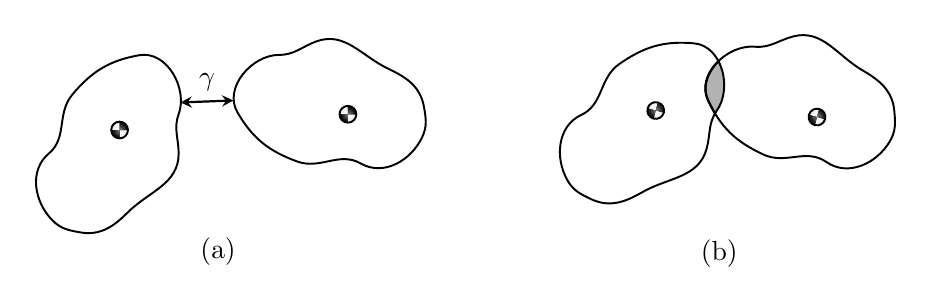
\begin{tikzpicture}[scale=\SF]
    \begin{scope}[scale=0.5]
        \draw[black,line width=0.7pt] (-1.2,1) to[out=50,in=190] (0.5,2) to[out=10,in=70] (1.5,0.5)
        to[out=-110,in=90] (1.5,-0.5) to[out=-90,in=45] (0.2,-2) to[out=-135,in=-10] (-1,-2.5) to[out=170,in=-45] (-1.7,-2.2) to[out=135,in=-140] (-1.8,-0.5) to[out=40,in=-130] (-1.2,1);
        \CoM{0}{0.1cm}{2mm};

        \draw[rotate=110,xshift=-1cm,yshift=-5cm,black,line width=0.7pt] (-1.2,1) to[out=50,in=190] (0.5,2) to[out=10,in=70] (1.5,0.5)
        to[out=-110,in=90] (1.5,-0.5) to[out=-90,in=45] (0.2,-2) to[out=-135,in=-10] (-1,-2.5) to[out=170,in=-45] (-1.7,-2.2) to[out=135,in=-140] (-1.8,-0.5) to[out=40,in=-130] (-1.2,1);
        \CoM{5.8cm}{0.5cm}{2mm};

        \draw[>=stealth,<->,thick] (1.55,0.8) -- node[pos=0.5,above]{\TS $\gamma$} (2.89,0.85);
        \draw (2.5,-3) node{\TS (a)};
    \end{scope}

    \begin{scope}[rotate=-15,scale=0.5,xshift=13cm,yshift=4cm]
        \begin{scope}
            \clip (-1.2,1) to[out=50,in=190] (0.5,2) to[out=10,in=70] (1.5,0.5)
        to[out=-110,in=90] (1.5,-0.5) to[out=-90,in=45] (0.2,-2) to[out=-135,in=-10] (-1,-2.5) to[out=170,in=-45] (-1.7,-2.2) to[out=135,in=-140] (-1.8,-0.5) to[out=40,in=-130] (-1.2,1);
            \filldraw[rotate=120,xshift=-0.5cm,yshift=-3.4cm,fill=black!30,draw=black,thick] (-1.2,1) to[out=50,in=190] (0.5,2) to[out=10,in=70] (1.5,0.5) to[out=-110,in=90] (1.5,-0.5) to[out=-90,in=45] (0.2,-2) to[out=-135,in=-10] (-1,-2.5) to[out=170,in=-45] (-1.7,-2.2) to[out=135,in=-140] (-1.8,-0.5) to[out=40,in=-130] (-1.2,1);
        \end{scope}

        \draw[black,line width=0.7pt] (-1.2,1) to[out=50,in=190] (0.5,2) to[out=10,in=70] (1.5,0.5)
        to[out=-110,in=90] (1.5,-0.5) to[out=-90,in=45] (0.2,-2) to[out=-135,in=-10] (-1,-2.5) to[out=170,in=-45] (-1.7,-2.2) to[out=135,in=-140] (-1.8,-0.5) to[out=40,in=-130] (-1.2,1);
        \CoM{0}{0.1cm}{2mm};

        \draw[rotate=120,xshift=-0.5cm,yshift=-3.4cm,black,line width=0.7pt] (-1.2,1) to[out=50,in=190] (0.5,2) to[out=10,in=70] (1.5,0.5)
        to[out=-110,in=90] (1.5,-0.5) to[out=-90,in=45] (0.2,-2) to[out=-135,in=-10] (-1,-2.5) to[out=170,in=-45] (-1.7,-2.2) to[out=135,in=-140] (-1.8,-0.5) to[out=40,in=-130] (-1.2,1);
        \CoM{4cm}{1cm}{2mm};

        \draw (2.5,-3) node{\TS (b)};
    \end{scope}
\end{tikzpicture}
\caption{This is the current style and layout of a figure caption.}
    \label{fig: chap1 impact bodies}
\end{figure}

\lipsum[19-23]



\subsection{Name of second subsection}\label{subsec: chap1 background3}

\lipsum[1-5]

%\newpage
\section{Problem statement}\label{sec: chap1 prob statement}

\lipsum[6-8]
Summarizing, the objective of the research is:
\vspace*{3mm}
\objective{State the objective of your PhD research here.}


\section{Research challenges and contributions}\label{sec: chap1 contributions}
In this section, the research problem is divided in ... research challenges with the topics: topic 1, topic 2, topic 3, ... . Per research challenge, a contribution of this thesis addressing the subproblem is presented.

%**********************************************************************%

\itemheader{Topic 1}
\lipsum[1-2] This leads to the first contribution of our work:

\contribution{First contribution of your work.}{\label{contr: contribution 1}}

Explain a bit more about your first contribution.

%**********************************************************************%

\itemheader{Topic 2}
\lipsum[4-5] This leads to the second contribution of our work:

\contribution{Second contribution of your work.}{\label{contr: contribution 2}}

Explain a bit more about your second contribution.

%**********************************************************************%

\itemheader{Topic 3}
\lipsum[1-2] The last contribution of the research thus is:

\contribution{Third contribution of your work.}{\label{contr: contribution 3}}

Explain a bit more about your third contribution.


\section{Outline of the thesis}\label{sec: chap1 outline}

\lipsum[10-12]

\itemheaderNewpage{A note for the reader} Chapters~...-... are all based on submitted/published articles and consequently are self-contained and can be read independently. A reference to the corresponding research paper is included at the beginning of each chapter.
An overview of how the chapters of this thesis relate to the contributions presented in Section~\ref{sec: chap1 contributions} is given in Table~...



% ------------------- FIRST PART -------------------%
\cleardoublepage
\part{Second chapter}\label{part: design}
\chapter{Title of the chapter}\label{chap: chapter 1}

\blfootnote{This chapter is based on:\\ write down the citation of the paper you are referring to in full.\disclaimer}


\chapterabstract{\lipsum[1]}

\section{Introduction} \label{sec: chap2 intro}
Showing footnotes still work even though we use blank footnotes\footnote{You see?}
\lipsum[5-7]

\section{Section header}\label{sec: chap2 section header}

Here's an equation:
\begin{equation}\label{eq: chap2 vector field} 
x = 1
\end{equation}

with $x$ the input, $t_0$ the initial time, and $t_f$ the final time. 
And below another beautiful image.



\section{Conclusions and discussion}
\label{sec: chap2 conclusion}

\lipsum[10-13]




% ------------------- SECOND PART -------------------%
\cleardoublepage
\part{Third part}\label{part: something}
%!TEX root = ../../thesis.tex
\chapter[Title of your chapter here]{Title of your chapter here}\label{chap: chapter 3}

\blfootnote{This chapter is based on:\\ write down the citation of the paper you are referring to in full.\disclaimer}

\chapterabstract{\lipsum[1]}

\section{Introduction}
\label{sec: chap3 intro}

\lipsum[5-7]


\section{Section header}
\label{sec: chap3 section header}

Here's an equation:
\begin{equation}\label{eq: chap3 vector field} 
x=2
\end{equation}
with $x\in y$ the input, $t_0$ the initial time, and $t_f$ the final time.
And below another beautiful image.

\begin{asm}[Roundeness of the earth]
We assume the earth is round because we like to believe that is true.
\end{asm}



\section{Conclusions and discussion}
\label{sec: chap3 conclusion}

\lipsum[10-13]


% ------------------- THIRD PART -------------------%
\part{Closing}\label{part: closing}
\chapter{Conclusions and recommendations}
\label{chap: conclusions}
\thispagestyle{empty}

\section{Conclusions}

\lipsum[20-23]
Restate your thesis objective.

\vspace*{3mm}
\objective{State the objective of your PhD research here.}



%**********************************************************************%


\section{Recommendations}

\lipsum[1-4]

% -------------------- APPENDIX --------------------%
\part{Appendices}\label{part: Appendices}
\appendix
\cleardoublepage

\definecolor{thumbcolor}{gray}{0.4}     % Change the color of the thumb index tags to gray
\chapter{Appendix name}
\label{app: appendix 1}

\section{Section header}

\lipsum[1-4]

% ------------------- BACK PART -------------------%
\placethumbfalse   % Stop putting thumbs from this point onwards
\bookmarksetup{startatroot}
\addtocontents{toc}{\bigskip}%

% -------------- BIBLIOGRAPHY ------------ %
{\fontsize{9pt}{10pt}\selectfont
\bibliographystyle{IEEEtran}
\cleardoublepage
\phantomsection
\addcontentsline{toc}{chapter}{\bibname}
\bibliography{src/bibliography}
% \nobibliography{src/bibliography}

}

% -------------- MODIFICATIONS ------------- %
\chapter*{Modifications}\label{chap: Modifications}
\addcontentsline{toc}{chapter}{Modifications}
\markboth{Modifications}{Modifications}

The chapters of your thesis are likely based on publications. In this chapter you can put the modifications with respect to those publications in forming the thesis content.

\section*{Overall modifications}
\begin{itemize}
    \item Phrases like \textit{this work}, \textit{this paper}, and \textit{this manuscript} are replaced by \textit{this chapter}, or \textit{this thesis}
\end{itemize}

\section*{Modifications Chapter 2}
\begin{itemize}
    \item A modification
    \item Another modification
\end{itemize}


% ------------- ACKNOWLEDGEMENT ------------ %
\normalsize
%*********************************************************************************%
\chapter*{Acknowledgements}
\addcontentsline{toc}{chapter}{Acknowledgements}
\markboth{Acknowledgements}{Acknowledgements}

\lipsum[14-18]



% --------------- PUBLICATIONS ------------- %
\newpage
%!TEX root = ../thesis.tex
\chapter*{List of publications}
\addcontentsline{toc}{chapter}{List of publications}
\markboth{List of publications}{List of publications}
\newcommand{\ipj}{(\textit{in preparation for journal submission})}
\newcommand{\cur}{(\textit{under review})}
\newcommand{\sbm}{(\textit{submitted})}
\newcommand{\acp}{(\textit{accepted})}
\newcommand{\inp}{(\textit{in press})}


%You think this can be done way easier with something like "bibentry" via the "bibentry" package.
%However, this also puts all references in the bibliography, which does not make sense if you don't 
%cite them... so only work around possible at this moment, is doing it manually :)

% -------------------------------- Journal papers -------------------------------- %
\begin{itemize}[leftmargin=4mm]
  \item B. Caasenbrood, A. Pogromsky and H. Nijmeijer, “\textit{Generative Design of Soft Robotic Actuators -- a Gradient-based Approach}”, Frontiers in Robotics and AI, 2022. \ipj;
\item B. Caasenbrood, A. Pogromsky and H. Nijmeijer, “\textit{Reduced-order Cosserat Models for Soft Robotic
 Systems using FEM-driven Shape Reconstruction}”, Robotics and Automation Letters, 2022. \ipj;
\item A. Amiri, B. Caasenbrood, D. Liu, N. van de Wouw, and I. Lopez Arteaga, "\textit{An Electric Circuit Model for the Nonlinear Dynamics of Electro-active Liquid Crystal Coatings}", Applied Physics Letters, 2022. \sbm;
\item  B. Caasenbrood, A. Pogromsky and H. Nijmeijer, “\textit{Energy-shaping Controllers for Soft Robot Manipulators through Port-Hamiltonian Cosserat Models}”, SN Computer Science Springer, 2022. \acp;
\item B. Caasenbrood, A. Pogromsky and H. Nijmeijer, "\textit{Control-oriented Models for Hyper-elastic Soft Robots through Differential Geometry of Curves}”, Soft Robotics, 2022. \inp
\end{itemize}

% ------------------------------ Conference papers ------------------------------ %
\section*{Peer-reviewed articles in conference proceedings}
\begin{itemize}[leftmargin=4mm]
\item B. Caasenbrood, F.E. van Beek, H. Khanh Chu, and I.A. Kuling, “\textit{A Desktop-sized Platform for Real-time Control Applications of Pneumatic Soft Robots},” IEEE International Conference on Soft Robotics, RoboSoft 2022, pp 217-223.
\item A. Amoozandeh Nobaveh, and B. Caasenbrood, "\textit{Design Feasibility of an Energy-efficient Wrist Exoskeleton
using Compliant Beams and Soft Actuators}", Proceedings of the 18th International  Consortium for Rehabilitation Robotics, 2022 (accepted).
\item B. Caasenbrood, A. Pogromsky and H. Nijmeijer, "\textit{Energy-based control for Soft Robots using Cosserat-beam models}”, Proceedings of the 18th International Conference on Informatics in Control, Automation and Robotics, 2021, pp. 311–319.
\item B. Caasenbrood, A. Pogromsky and H. Nijmeijer, "\textit{A Computational Design Framework for Pressure-driven Soft Robots through Nonlinear Topology Optimization}," 2020 3rd IEEE International Conference on Soft Robotics, 2020, pp. 633-638.
\item B. Caasenbrood, A. Pogromsky and H. Nijmeijer, “\textit{Dynamic modeling of hyper-elastic soft robots using spatial curves},” IFAC World Congress, IFAC-PapersOnLine, 2020, pp. 9238-9243.
\end{itemize}


% ---------------- Invited talks and Non Peer-reviewed Abstracts ---------------- %
\section*{Invited Talks and Non Peer-reviewed Abstracts}
\begin{itemize}[leftmargin=4mm]
\item B. Caasenbrood, “\texttt{SOROTOKI}\textit{: an Open-source Toolkit for Soft Robotics written in MATLAB},”  IEEE International Conference on Soft Robotics, RoboSoft 2022 (abstract). \texttt{Best Poster Award}
\item B. Caasenbrood, C. Della Santina, and A. Pogromsky, “\textit{Workshop on Model-based Control of Soft Robots},” European Control Conference (ECC), 2021. (main organizer).
\item B. Caasenbrood, talk on  “\textit{Towards Desing and Control of Soft Robotics},” 4TU Symposium on Soft Robotics, 2020. (invited speaker).
\item B. Caasenbrood, talk on  “\textit{3D-printed Soft Robotics},” Symposium on Robotic Technologies, 2019. (invited speaker).
\item B. Caasenbrood, A. Pogromsky and H. Nijmeijer, talk on  “\textit{Forward Dynamics of Hyper-elastic Soft Robotics},” 39th Benelux Meeting on Systems and Control, 2019. (abstract).
\item B. Caasenbrood, A. Pogromsky and H. Nijmeijer, talk on  “\textit{Dynamical modeling and control of continuum soft robots},” 37th Benelux Meeting on Systems and Control, 2018. (abstract).
\end{itemize}

% -------------------- CV ------------------ %
%*********************************************************************************%
% \chapter*{Curriculum Vitae}
% \addcontentsline{toc}{chapter}{Curriculum Vitae}
% \markboth{Curriculum Vitae}{Curriculum Vitae}

\chapter*{About the author}
\addcontentsline{toc}{chapter}{About the author}
\markboth{About the author}{About the author}


\begin{wrapfigure}{l}{0.25\textwidth}
    \centering
    
\includegraphics[width=0.25\textwidth]{img/authorpicture.jpg}
\end{wrapfigure}

\lipsum[5-7]


\thispagestyle{empty}

\ifprint{}
\else
\newpage {~}
\thispagestyle{empty}
\fi

%%%% BACK **********************************************************************
% \cover{thesis_back.pdf}    % Adds your thesis' back cover if the option 'print' is NOT used. Printing companies require the thesis cover to be supplied separately and in a different format. Definition of \cover{} is given in commands.tex.

\end{document}